In this chapter, we will examine the state of art of \textbf{computer graphics}. Our aim is to understand techniques which are actually used for visualization of the three-dimensional biomedical models, and to provide a basis for comprehension of the innovative approaches we will show further on. A lot of this material comes from \cite{Hughes}, which is a classic book for this field\\

Here, we will also show the actual techniques used for the generation of volumes and surfaces from the biomedical images so we will see the difference with our approach 

\section{Representation of shapes in graphics: meshes}\label{sec14:mesh}

The first thing we will examine is the most widely used representation of shapes in graphics: \textbf{meshes}. At first we will focus on \textit{triangle meshes} but we could define meshes with $n$ vertices. Triangle meshes simply consist of many triangles joined along their vertices to form a surface. They have some interesting properties, but the most important is \textbf{coplanarity} of vertices of a single triangle.

\begin{figure}[htb] %  figure placement: here, top, bottom
   \centering
   % Graphic for TeX using PGF
% Title: /media/danilo/E472BA7972BA5052/Danilo/Documenti/Università/LatexTesiMagistrale/images/meshes.dia
% Creator: Dia v0.97.3
% CreationDate: Fri Jan 29 10:28:45 2016
% For: danilo
% \usepackage{tikz}
% The following commands are not supported in PSTricks at present
% We define them conditionally, so when they are implemented,
% this pgf file will use them.
\ifx\du\undefined
  \newlength{\du}
\fi
\setlength{\du}{15\unitlength}
\begin{tikzpicture}
\pgftransformxscale{1.000000}
\pgftransformyscale{-1.000000}
\definecolor{dialinecolor}{rgb}{0.000000, 0.000000, 0.000000}
\pgfsetstrokecolor{dialinecolor}
\definecolor{dialinecolor}{rgb}{1.000000, 1.000000, 1.000000}
\pgfsetfillcolor{dialinecolor}
\pgfsetlinewidth{0.050000\du}
\pgfsetdash{}{0pt}
\pgfsetdash{}{0pt}
\pgfsetmiterjoin
\pgfsetbuttcap
\definecolor{dialinecolor}{rgb}{0.952941, 0.839216, 0.929412}
\pgfsetfillcolor{dialinecolor}
\fill (18.000000\du,5.000000\du)--(21.000000\du,5.000000\du)--(20.000000\du,9.000000\du)--cycle;
\definecolor{dialinecolor}{rgb}{0.000000, 0.000000, 0.000000}
\pgfsetstrokecolor{dialinecolor}
\draw (18.000000\du,5.000000\du)--(21.000000\du,5.000000\du)--(20.000000\du,9.000000\du)--cycle;
\pgfsetlinewidth{0.050000\du}
\pgfsetdash{}{0pt}
\pgfsetdash{}{0pt}
\pgfsetmiterjoin
\pgfsetbuttcap
\definecolor{dialinecolor}{rgb}{0.600000, 1.000000, 0.600000}
\pgfsetfillcolor{dialinecolor}
\fill (21.000000\du,5.000000\du)--(25.000000\du,5.000000\du)--(22.000000\du,3.000000\du)--cycle;
\definecolor{dialinecolor}{rgb}{0.000000, 0.000000, 0.000000}
\pgfsetstrokecolor{dialinecolor}
\draw (21.000000\du,5.000000\du)--(25.000000\du,5.000000\du)--(22.000000\du,3.000000\du)--cycle;
\pgfsetlinewidth{0.050000\du}
\pgfsetdash{}{0pt}
\pgfsetdash{}{0pt}
\pgfsetmiterjoin
\pgfsetbuttcap
\definecolor{dialinecolor}{rgb}{0.584314, 0.772549, 0.788235}
\pgfsetfillcolor{dialinecolor}
\fill (18.000000\du,5.000000\du)--(21.000000\du,5.000000\du)--(19.000000\du,3.000000\du)--cycle;
\definecolor{dialinecolor}{rgb}{0.000000, 0.000000, 0.000000}
\pgfsetstrokecolor{dialinecolor}
\draw (18.000000\du,5.000000\du)--(21.000000\du,5.000000\du)--(19.000000\du,3.000000\du)--cycle;
\pgfsetlinewidth{0.050000\du}
\pgfsetdash{}{0pt}
\pgfsetdash{}{0pt}
\pgfsetmiterjoin
\pgfsetbuttcap
\definecolor{dialinecolor}{rgb}{1.000000, 0.000000, 0.000000}
\pgfsetfillcolor{dialinecolor}
\fill (19.000000\du,3.000000\du)--(22.000000\du,3.000000\du)--(21.000000\du,5.000000\du)--cycle;
\definecolor{dialinecolor}{rgb}{0.000000, 0.000000, 0.000000}
\pgfsetstrokecolor{dialinecolor}
\draw (19.000000\du,3.000000\du)--(22.000000\du,3.000000\du)--(21.000000\du,5.000000\du)--cycle;
\pgfsetlinewidth{0.050000\du}
\pgfsetdash{}{0pt}
\pgfsetdash{}{0pt}
\pgfsetmiterjoin
\pgfsetbuttcap
\definecolor{dialinecolor}{rgb}{1.000000, 0.996078, 0.521569}
\pgfsetfillcolor{dialinecolor}
\fill (21.000000\du,5.000000\du)--(25.000000\du,5.000000\du)--(23.000000\du,10.000000\du)--cycle;
\definecolor{dialinecolor}{rgb}{0.000000, 0.000000, 0.000000}
\pgfsetstrokecolor{dialinecolor}
\draw (21.000000\du,5.000000\du)--(25.000000\du,5.000000\du)--(23.000000\du,10.000000\du)--cycle;
\pgfsetlinewidth{0.050000\du}
\pgfsetdash{}{0pt}
\pgfsetdash{}{0pt}
\pgfsetmiterjoin
\pgfsetbuttcap
\definecolor{dialinecolor}{rgb}{0.847059, 0.898039, 0.898039}
\pgfsetfillcolor{dialinecolor}
\fill (20.000000\du,9.000000\du)--(21.000000\du,5.000000\du)--(23.000000\du,10.000000\du)--cycle;
\definecolor{dialinecolor}{rgb}{0.000000, 0.000000, 0.000000}
\pgfsetstrokecolor{dialinecolor}
\draw (20.000000\du,9.000000\du)--(21.000000\du,5.000000\du)--(23.000000\du,10.000000\du)--cycle;
\pgfsetlinewidth{0.050000\du}
\pgfsetdash{}{0pt}
\pgfsetdash{}{0pt}
\pgfsetmiterjoin
\pgfsetbuttcap
\definecolor{dialinecolor}{rgb}{1.000000, 0.996078, 0.521569}
\pgfsetfillcolor{dialinecolor}
\fill (28.000000\du,5.000000\du)--(32.000000\du,9.000000\du)--(28.000000\du,9.000000\du)--cycle;
\definecolor{dialinecolor}{rgb}{0.000000, 0.000000, 0.000000}
\pgfsetstrokecolor{dialinecolor}
\draw (28.000000\du,5.000000\du)--(32.000000\du,9.000000\du)--(28.000000\du,9.000000\du)--cycle;
\pgfsetlinewidth{0.050000\du}
\pgfsetdash{}{0pt}
\pgfsetdash{}{0pt}
\pgfsetmiterjoin
\pgfsetbuttcap
\definecolor{dialinecolor}{rgb}{0.847059, 0.898039, 0.898039}
\pgfsetfillcolor{dialinecolor}
\fill (28.000000\du,5.000000\du)--(32.000000\du,9.000000\du)--(32.000000\du,5.000000\du)--cycle;
\definecolor{dialinecolor}{rgb}{0.000000, 0.000000, 0.000000}
\pgfsetstrokecolor{dialinecolor}
\draw (28.000000\du,5.000000\du)--(32.000000\du,9.000000\du)--(32.000000\du,5.000000\du)--cycle;
\pgfsetlinewidth{0.050000\du}
\pgfsetdash{}{0pt}
\pgfsetdash{}{0pt}
\pgfsetmiterjoin
\pgfsetbuttcap
\definecolor{dialinecolor}{rgb}{0.952941, 0.839216, 0.929412}
\pgfsetfillcolor{dialinecolor}
\fill (30.000000\du,3.000000\du)--(32.000000\du,5.000000\du)--(34.000000\du,3.000000\du)--cycle;
\definecolor{dialinecolor}{rgb}{0.000000, 0.000000, 0.000000}
\pgfsetstrokecolor{dialinecolor}
\draw (30.000000\du,3.000000\du)--(32.000000\du,5.000000\du)--(34.000000\du,3.000000\du)--cycle;
\pgfsetlinewidth{0.050000\du}
\pgfsetdash{}{0pt}
\pgfsetdash{}{0pt}
\pgfsetmiterjoin
\pgfsetbuttcap
\definecolor{dialinecolor}{rgb}{0.600000, 1.000000, 0.600000}
\pgfsetfillcolor{dialinecolor}
\fill (30.000000\du,3.000000\du)--(28.000000\du,5.000000\du)--(32.000000\du,5.000000\du)--cycle;
\definecolor{dialinecolor}{rgb}{0.000000, 0.000000, 0.000000}
\pgfsetstrokecolor{dialinecolor}
\draw (30.000000\du,3.000000\du)--(28.000000\du,5.000000\du)--(32.000000\du,5.000000\du)--cycle;
\pgfsetlinewidth{0.050000\du}
\pgfsetdash{}{0pt}
\pgfsetdash{}{0pt}
\pgfsetmiterjoin
\pgfsetbuttcap
\definecolor{dialinecolor}{rgb}{0.909804, 0.698039, 0.560784}
\pgfsetfillcolor{dialinecolor}
\fill (32.000000\du,9.000000\du)--(34.000000\du,6.800000\du)--(32.000000\du,5.000000\du)--cycle;
\definecolor{dialinecolor}{rgb}{0.000000, 0.000000, 0.000000}
\pgfsetstrokecolor{dialinecolor}
\draw (32.000000\du,9.000000\du)--(34.000000\du,6.800000\du)--(32.000000\du,5.000000\du)--cycle;
\pgfsetlinewidth{0.050000\du}
\pgfsetdash{}{0pt}
\pgfsetdash{}{0pt}
\pgfsetmiterjoin
\pgfsetbuttcap
\definecolor{dialinecolor}{rgb}{1.000000, 0.000000, 0.000000}
\pgfsetfillcolor{dialinecolor}
\fill (34.000000\du,3.000000\du)--(34.000000\du,6.800000\du)--(32.000000\du,5.000000\du)--cycle;
\definecolor{dialinecolor}{rgb}{0.000000, 0.000000, 0.000000}
\pgfsetstrokecolor{dialinecolor}
\draw (34.000000\du,3.000000\du)--(34.000000\du,6.800000\du)--(32.000000\du,5.000000\du)--cycle;
\end{tikzpicture}

   \caption[Examples of triangular meshes]{Creation of shapes with composition of triangular meshes. As we can see using this composition we can create whichever shape we want. At the same time we can decompose every complex shape into triangles}
   \label{fig:triangularMeshes}
\end{figure}

Two interesting operations on meshes are \textit{subdivision} (where a single triangle is replaced with several small triangles for smoothing a shape) and \textit{simplification} (when a mesh is replaced with another that is similar but has a more compact representation). As a consequence of these properties and operations, we are able to represent whichever shape approximating it with triangles (see Figure~\ref{fig:triangularMeshes}), we will have an evidence of this when we will see models from our application.\\

Now we can focus on the representation of three-dimensional meshes. The simpler data structure (and the one we will use later) for description of these meshes consists in a \textit{list of vertices} and in a \textit{list of triangles}. With this structure we can also infer edges of the meshes using topological techniques. With this structure, insertion of triangles and vertices is fast ($O(1)$) but deletion of vertices is slow (it is $O(n)$ because we need to find all associated triangles).

\subsection{Manifold and Nonmanifold meshes}
Some particular meshes are the \textbf{manifold meshes}. According to \cite{Hughes}, we can introduce the following definition:

\begin{definition}[Manifold meshes]
A finite 2D mesh is a manifold mesh if the edges and triangles meeting a vertex $v$ can be arranged in a cyclic order\\ $t_{1}, e_{1}, t_{2}, e_{2}, \dots, t_{n}, e_{n}$ without repetitions such that edge $e_{i}$ is an edge of triangles $t_{i}$ and $t_{i+1}$
\end{definition}

This implies that for a manifold mesh every edge is \textit{incident with at most two faces}. These structures are central to many parts of geometry and modern mathematical physics because they allows more complicated structures to be described and understood in terms of the relatively well-understood properties of Euclidean space.\\

Often, we should care about the orientation of triangles in a mesh (for example when we consider lighting). In fact, orientation is fundamental when we want to find the \textit{normal vector} of the face and decide what is inside and what is outside our meshes. Moreover, when two adjacent triangles have consistently oriented normal vectors, then the edge they share will appear as $(i, j)$ in one triangle and as $(j, i)$ in the other. And if a manifold mesh can have its triangles oriented, it can also be given consistently oriented normal vectors.\\

\begin{figure}[htb] %  figure placement: here, top, bottom
   \centering
   % Graphic for TeX using PGF
% Title: /media/danilo/E472BA7972BA5052/Danilo/Documenti/Università/LatexTesiMagistrale/images/normals.dia
% Creator: Dia v0.97.3
% CreationDate: Fri Jan 29 15:14:30 2016
% For: danilo
% \usepackage{tikz}
% The following commands are not supported in PSTricks at present
% We define them conditionally, so when they are implemented,
% this pgf file will use them.
\ifx\du\undefined
  \newlength{\du}
\fi
\setlength{\du}{15\unitlength}
\begin{tikzpicture}
\pgftransformxscale{1.000000}
\pgftransformyscale{-1.000000}
\definecolor{dialinecolor}{rgb}{0.000000, 0.000000, 0.000000}
\pgfsetstrokecolor{dialinecolor}
\definecolor{dialinecolor}{rgb}{1.000000, 1.000000, 1.000000}
\pgfsetfillcolor{dialinecolor}
\pgfsetlinewidth{0.010000\du}
\pgfsetdash{}{0pt}
\pgfsetdash{}{0pt}
\pgfsetmiterjoin
\pgfsetbuttcap
\definecolor{dialinecolor}{rgb}{0.847059, 0.898039, 0.898039}
\pgfsetfillcolor{dialinecolor}
\fill (16.000000\du,5.000000\du)--(18.000000\du,2.000000\du)--(19.000000\du,7.000000\du)--cycle;
\definecolor{dialinecolor}{rgb}{0.000000, 0.000000, 0.000000}
\pgfsetstrokecolor{dialinecolor}
\draw (16.000000\du,5.000000\du)--(18.000000\du,2.000000\du)--(19.000000\du,7.000000\du)--cycle;
\pgfsetlinewidth{0.010000\du}
\pgfsetdash{}{0pt}
\pgfsetdash{}{0pt}
\pgfsetmiterjoin
\pgfsetbuttcap
\definecolor{dialinecolor}{rgb}{0.847059, 0.898039, 0.898039}
\pgfsetfillcolor{dialinecolor}
\fill (18.000000\du,2.000000\du)--(22.000000\du,1.000000\du)--(19.000000\du,7.000000\du)--cycle;
\definecolor{dialinecolor}{rgb}{0.000000, 0.000000, 0.000000}
\pgfsetstrokecolor{dialinecolor}
\draw (18.000000\du,2.000000\du)--(22.000000\du,1.000000\du)--(19.000000\du,7.000000\du)--cycle;
\pgfsetlinewidth{0.010000\du}
\pgfsetdash{}{0pt}
\pgfsetdash{}{0pt}
\pgfsetmiterjoin
\pgfsetbuttcap
\definecolor{dialinecolor}{rgb}{0.847059, 0.898039, 0.898039}
\pgfsetfillcolor{dialinecolor}
\fill (22.000000\du,1.000000\du)--(26.000000\du,5.000000\du)--(19.000000\du,7.000000\du)--cycle;
\definecolor{dialinecolor}{rgb}{0.000000, 0.000000, 0.000000}
\pgfsetstrokecolor{dialinecolor}
\draw (22.000000\du,1.000000\du)--(26.000000\du,5.000000\du)--(19.000000\du,7.000000\du)--cycle;
\pgfsetlinewidth{0.050000\du}
\pgfsetdash{}{0pt}
\pgfsetdash{}{0pt}
\pgfsetbuttcap
{
\definecolor{dialinecolor}{rgb}{0.000000, 0.000000, 0.000000}
\pgfsetfillcolor{dialinecolor}
% was here!!!
\pgfsetarrowsend{stealth}
\definecolor{dialinecolor}{rgb}{0.000000, 0.000000, 0.000000}
\pgfsetstrokecolor{dialinecolor}
\pgfpathmoveto{\pgfpoint{19.920820\du}{2.700220\du}}
\pgfpatharc{278}{97}{0.629947\du and 0.629947\du}
\pgfusepath{stroke}
}
\pgfsetlinewidth{0.050000\du}
\pgfsetdash{}{0pt}
\pgfsetdash{}{0pt}
\pgfsetbuttcap
{
\definecolor{dialinecolor}{rgb}{0.000000, 0.000000, 0.000000}
\pgfsetfillcolor{dialinecolor}
% was here!!!
\pgfsetarrowsend{stealth}
\definecolor{dialinecolor}{rgb}{0.000000, 0.000000, 0.000000}
\pgfsetstrokecolor{dialinecolor}
\pgfpathmoveto{\pgfpoint{21.542546\du}{4.873097\du}}
\pgfpatharc{147}{-72}{0.516414\du and 0.516414\du}
\pgfusepath{stroke}
}
\pgfsetlinewidth{0.050000\du}
\pgfsetdash{}{0pt}
\pgfsetdash{}{0pt}
\pgfsetbuttcap
{
\definecolor{dialinecolor}{rgb}{0.000000, 0.000000, 0.000000}
\pgfsetfillcolor{dialinecolor}
% was here!!!
\pgfsetarrowsend{stealth}
\definecolor{dialinecolor}{rgb}{0.000000, 0.000000, 0.000000}
\pgfsetstrokecolor{dialinecolor}
\pgfpathmoveto{\pgfpoint{17.258784\du}{5.344409\du}}
\pgfpatharc{134}{-87}{0.510822\du and 0.510822\du}
\pgfusepath{stroke}
}
% setfont left to latex
\definecolor{dialinecolor}{rgb}{0.000000, 0.000000, 0.000000}
\pgfsetstrokecolor{dialinecolor}
\node[anchor=west] at (17.719480\du,1.497234\du){1};
% setfont left to latex
\definecolor{dialinecolor}{rgb}{0.000000, 0.000000, 0.000000}
\pgfsetstrokecolor{dialinecolor}
\node[anchor=west] at (18.774015\du,7.728495\du){2};
% setfont left to latex
\definecolor{dialinecolor}{rgb}{0.000000, 0.000000, 0.000000}
\pgfsetstrokecolor{dialinecolor}
\node[anchor=west] at (22.006396\du,0.736466\du){3};
\pgfsetlinewidth{0.010000\du}
\pgfsetdash{}{0pt}
\pgfsetdash{}{0pt}
\pgfsetmiterjoin
\pgfsetbuttcap
\definecolor{dialinecolor}{rgb}{0.847059, 0.898039, 0.898039}
\pgfsetfillcolor{dialinecolor}
\fill (29.000000\du,5.000000\du)--(31.000000\du,2.000000\du)--(32.000000\du,7.000000\du)--cycle;
\definecolor{dialinecolor}{rgb}{0.000000, 0.000000, 0.000000}
\pgfsetstrokecolor{dialinecolor}
\draw (29.000000\du,5.000000\du)--(31.000000\du,2.000000\du)--(32.000000\du,7.000000\du)--cycle;
\pgfsetlinewidth{0.010000\du}
\pgfsetdash{}{0pt}
\pgfsetdash{}{0pt}
\pgfsetmiterjoin
\pgfsetbuttcap
\definecolor{dialinecolor}{rgb}{0.847059, 0.898039, 0.898039}
\pgfsetfillcolor{dialinecolor}
\fill (31.000000\du,2.000000\du)--(35.000000\du,1.000000\du)--(32.000000\du,7.000000\du)--cycle;
\definecolor{dialinecolor}{rgb}{0.000000, 0.000000, 0.000000}
\pgfsetstrokecolor{dialinecolor}
\draw (31.000000\du,2.000000\du)--(35.000000\du,1.000000\du)--(32.000000\du,7.000000\du)--cycle;
\pgfsetlinewidth{0.010000\du}
\pgfsetdash{}{0pt}
\pgfsetdash{}{0pt}
\pgfsetmiterjoin
\pgfsetbuttcap
\definecolor{dialinecolor}{rgb}{0.847059, 0.898039, 0.898039}
\pgfsetfillcolor{dialinecolor}
\fill (35.000000\du,1.000000\du)--(39.000000\du,5.000000\du)--(32.000000\du,7.000000\du)--cycle;
\definecolor{dialinecolor}{rgb}{0.000000, 0.000000, 0.000000}
\pgfsetstrokecolor{dialinecolor}
\draw (35.000000\du,1.000000\du)--(39.000000\du,5.000000\du)--(32.000000\du,7.000000\du)--cycle;
% setfont left to latex
\definecolor{dialinecolor}{rgb}{0.000000, 0.000000, 0.000000}
\pgfsetstrokecolor{dialinecolor}
\node[anchor=west] at (30.860898\du,1.474746\du){1};
% setfont left to latex
\definecolor{dialinecolor}{rgb}{0.000000, 0.000000, 0.000000}
\pgfsetstrokecolor{dialinecolor}
\node[anchor=west] at (31.774015\du,7.728495\du){2};
% setfont left to latex
\definecolor{dialinecolor}{rgb}{0.000000, 0.000000, 0.000000}
\pgfsetstrokecolor{dialinecolor}
\node[anchor=west] at (35.006396\du,0.736466\du){3};
\pgfsetlinewidth{0.100000\du}
\pgfsetdash{}{0pt}
\pgfsetdash{}{0pt}
\pgfsetbuttcap
{
\definecolor{dialinecolor}{rgb}{0.000000, 0.000000, 0.000000}
\pgfsetfillcolor{dialinecolor}
% was here!!!
\pgfsetarrowsend{to}
\definecolor{dialinecolor}{rgb}{0.000000, 0.000000, 0.000000}
\pgfsetstrokecolor{dialinecolor}
\draw (30.500000\du,4.500000\du)--(28.855006\du,3.509326\du);
}
\pgfsetlinewidth{0.100000\du}
\pgfsetdash{}{0pt}
\pgfsetdash{}{0pt}
\pgfsetbuttcap
{
\definecolor{dialinecolor}{rgb}{0.000000, 0.000000, 0.000000}
\pgfsetfillcolor{dialinecolor}
% was here!!!
\pgfsetarrowsend{to}
\definecolor{dialinecolor}{rgb}{0.000000, 0.000000, 0.000000}
\pgfsetstrokecolor{dialinecolor}
\draw (33.000000\du,4.000000\du)--(33.026836\du,1.918374\du);
}
\pgfsetlinewidth{0.100000\du}
\pgfsetdash{}{0pt}
\pgfsetdash{}{0pt}
\pgfsetbuttcap
{
\definecolor{dialinecolor}{rgb}{0.000000, 0.000000, 0.000000}
\pgfsetfillcolor{dialinecolor}
% was here!!!
\pgfsetarrowsend{to}
\definecolor{dialinecolor}{rgb}{0.000000, 0.000000, 0.000000}
\pgfsetstrokecolor{dialinecolor}
\draw (35.500000\du,4.000000\du)--(37.481501\du,2.554755\du);
}
\end{tikzpicture}

   \caption[Meshes orientation and normals]{Meshes orientation and normals. As we can see in (a), for oriented faces we always have that for a common edge between two faces in the first we will have $(i, j)$ and in the second we will have $(j , i)$. In the example we can observe $(1, 2)$ and $(2, 1)$}
   \label{fig:normals}
\end{figure}

More interesting than manifold meshes are meshes whose vertices are manifold or \textbf{boundarylike}. In the last case, vertices do not form a cycle but a chain, whose first and last elements share only one of their edges with other triangles in the chain. The other edge of the first (or the last) triangle that meets the vertex is contained only in the first (or the last) triangle, and not in any other triangle of the mesh. This unshared edge is called a \textbf{boundary edge}, and the vertex is called a \textbf{boundary vertex}. In general, an oriented mesh without boundary edges is called \textbf{closed}

\begin{figure}[htb] %  figure placement: here, top, bottom
   \centering
   % Graphic for TeX using PGF
% Title: /media/danilo/E472BA7972BA5052/Danilo/Documenti/Università/LatexTesiMagistrale/images/boundarylike.dia
% Creator: Dia v0.97.3
% CreationDate: Fri Jan 29 15:39:12 2016
% For: danilo
% \usepackage{tikz}
% The following commands are not supported in PSTricks at present
% We define them conditionally, so when they are implemented,
% this pgf file will use them.
\ifx\du\undefined
  \newlength{\du}
\fi
\setlength{\du}{15\unitlength}
\begin{tikzpicture}
\pgftransformxscale{1.000000}
\pgftransformyscale{-1.000000}
\definecolor{dialinecolor}{rgb}{0.000000, 0.000000, 0.000000}
\pgfsetstrokecolor{dialinecolor}
\definecolor{dialinecolor}{rgb}{1.000000, 1.000000, 1.000000}
\pgfsetfillcolor{dialinecolor}
\pgfsetlinewidth{0.000000\du}
\pgfsetdash{}{0pt}
\pgfsetdash{}{0pt}
\pgfsetmiterjoin
\pgfsetbuttcap
\definecolor{dialinecolor}{rgb}{1.000000, 0.996078, 0.521569}
\pgfsetfillcolor{dialinecolor}
\fill (16.000000\du,2.000000\du)--(19.000000\du,1.000000\du)--(20.000000\du,4.000000\du)--cycle;
\definecolor{dialinecolor}{rgb}{0.000000, 0.000000, 0.000000}
\pgfsetstrokecolor{dialinecolor}
\draw (16.000000\du,2.000000\du)--(19.000000\du,1.000000\du)--(20.000000\du,4.000000\du)--cycle;
\pgfsetlinewidth{0.000000\du}
\pgfsetdash{}{0pt}
\pgfsetdash{}{0pt}
\pgfsetmiterjoin
\pgfsetbuttcap
\definecolor{dialinecolor}{rgb}{0.882353, 0.725490, 0.474510}
\pgfsetfillcolor{dialinecolor}
\fill (19.000000\du,1.000000\du)--(21.000000\du,0.000000\du)--(20.000000\du,4.000000\du)--cycle;
\definecolor{dialinecolor}{rgb}{0.000000, 0.000000, 0.000000}
\pgfsetstrokecolor{dialinecolor}
\draw (19.000000\du,1.000000\du)--(21.000000\du,0.000000\du)--(20.000000\du,4.000000\du)--cycle;
\pgfsetlinewidth{0.000000\du}
\pgfsetdash{}{0pt}
\pgfsetdash{}{0pt}
\pgfsetmiterjoin
\pgfsetbuttcap
\definecolor{dialinecolor}{rgb}{0.882353, 0.725490, 0.474510}
\pgfsetfillcolor{dialinecolor}
\fill (23.000000\du,2.000000\du)--(22.000000\du,7.000000\du)--(20.000000\du,4.000000\du)--cycle;
\definecolor{dialinecolor}{rgb}{0.000000, 0.000000, 0.000000}
\pgfsetstrokecolor{dialinecolor}
\draw (23.000000\du,2.000000\du)--(22.000000\du,7.000000\du)--(20.000000\du,4.000000\du)--cycle;
\pgfsetlinewidth{0.000000\du}
\pgfsetdash{}{0pt}
\pgfsetdash{}{0pt}
\pgfsetmiterjoin
\pgfsetbuttcap
\definecolor{dialinecolor}{rgb}{0.882353, 0.725490, 0.474510}
\pgfsetfillcolor{dialinecolor}
\fill (16.000000\du,2.000000\du)--(20.000000\du,4.000000\du)--(17.000000\du,6.000000\du)--cycle;
\definecolor{dialinecolor}{rgb}{0.000000, 0.000000, 0.000000}
\pgfsetstrokecolor{dialinecolor}
\draw (16.000000\du,2.000000\du)--(20.000000\du,4.000000\du)--(17.000000\du,6.000000\du)--cycle;
\pgfsetlinewidth{0.000000\du}
\pgfsetdash{}{0pt}
\pgfsetdash{}{0pt}
\pgfsetmiterjoin
\pgfsetbuttcap
\definecolor{dialinecolor}{rgb}{1.000000, 0.996078, 0.521569}
\pgfsetfillcolor{dialinecolor}
\fill (17.000000\du,6.000000\du)--(20.000000\du,4.000000\du)--(22.000000\du,7.000000\du)--cycle;
\definecolor{dialinecolor}{rgb}{0.000000, 0.000000, 0.000000}
\pgfsetstrokecolor{dialinecolor}
\draw (17.000000\du,6.000000\du)--(20.000000\du,4.000000\du)--(22.000000\du,7.000000\du)--cycle;
\pgfsetlinewidth{0.000000\du}
\pgfsetdash{}{0pt}
\pgfsetdash{}{0pt}
\pgfsetmiterjoin
\pgfsetbuttcap
\definecolor{dialinecolor}{rgb}{1.000000, 0.996078, 0.521569}
\pgfsetfillcolor{dialinecolor}
\fill (21.000000\du,0.000000\du)--(23.000000\du,2.000000\du)--(20.000000\du,4.000000\du)--cycle;
\definecolor{dialinecolor}{rgb}{0.000000, 0.000000, 0.000000}
\pgfsetstrokecolor{dialinecolor}
\draw (21.000000\du,0.000000\du)--(23.000000\du,2.000000\du)--(20.000000\du,4.000000\du)--cycle;
\pgfsetlinewidth{0.000000\du}
\pgfsetdash{}{0pt}
\pgfsetdash{}{0pt}
\pgfsetmiterjoin
\pgfsetbuttcap
\definecolor{dialinecolor}{rgb}{1.000000, 0.996078, 0.521569}
\pgfsetfillcolor{dialinecolor}
\fill (31.000000\du,7.000000\du)--(33.000000\du,5.000000\du)--(37.000000\du,7.000000\du)--cycle;
\definecolor{dialinecolor}{rgb}{0.000000, 0.000000, 0.000000}
\pgfsetstrokecolor{dialinecolor}
\draw (31.000000\du,7.000000\du)--(33.000000\du,5.000000\du)--(37.000000\du,7.000000\du)--cycle;
\pgfsetlinewidth{0.000000\du}
\pgfsetdash{}{0pt}
\pgfsetdash{}{0pt}
\pgfsetmiterjoin
\pgfsetbuttcap
\definecolor{dialinecolor}{rgb}{0.882353, 0.725490, 0.474510}
\pgfsetfillcolor{dialinecolor}
\fill (35.000000\du,4.000000\du)--(37.000000\du,7.000000\du)--(33.000000\du,5.000000\du)--cycle;
\definecolor{dialinecolor}{rgb}{0.000000, 0.000000, 0.000000}
\pgfsetstrokecolor{dialinecolor}
\draw (35.000000\du,4.000000\du)--(37.000000\du,7.000000\du)--(33.000000\du,5.000000\du)--cycle;
\pgfsetlinewidth{0.000000\du}
\pgfsetdash{}{0pt}
\pgfsetdash{}{0pt}
\pgfsetmiterjoin
\pgfsetbuttcap
\definecolor{dialinecolor}{rgb}{0.882353, 0.725490, 0.474510}
\pgfsetfillcolor{dialinecolor}
\fill (33.000000\du,5.000000\du)--(31.000000\du,7.000000\du)--(29.000000\du,5.000000\du)--cycle;
\definecolor{dialinecolor}{rgb}{0.000000, 0.000000, 0.000000}
\pgfsetstrokecolor{dialinecolor}
\draw (33.000000\du,5.000000\du)--(31.000000\du,7.000000\du)--(29.000000\du,5.000000\du)--cycle;
\pgfsetlinewidth{0.000000\du}
\pgfsetdash{}{0pt}
\pgfsetdash{}{0pt}
\pgfsetmiterjoin
\pgfsetbuttcap
\definecolor{dialinecolor}{rgb}{0.882353, 0.725490, 0.474510}
\pgfsetfillcolor{dialinecolor}
\fill (35.000000\du,4.000000\du)--(41.000000\du,5.000000\du)--(37.000000\du,7.000000\du)--cycle;
\definecolor{dialinecolor}{rgb}{0.000000, 0.000000, 0.000000}
\pgfsetstrokecolor{dialinecolor}
\draw (35.000000\du,4.000000\du)--(41.000000\du,5.000000\du)--(37.000000\du,7.000000\du)--cycle;
\pgfsetlinewidth{0.000000\du}
\pgfsetdash{}{0pt}
\pgfsetdash{}{0pt}
\pgfsetmiterjoin
\pgfsetbuttcap
\definecolor{dialinecolor}{rgb}{1.000000, 0.996078, 0.521569}
\pgfsetfillcolor{dialinecolor}
\fill (26.000000\du,7.000000\du)--(29.000000\du,5.000000\du)--(31.000000\du,7.000000\du)--cycle;
\definecolor{dialinecolor}{rgb}{0.000000, 0.000000, 0.000000}
\pgfsetstrokecolor{dialinecolor}
\draw (26.000000\du,7.000000\du)--(29.000000\du,5.000000\du)--(31.000000\du,7.000000\du)--cycle;
\pgfsetlinewidth{0.000000\du}
\pgfsetdash{}{0pt}
\pgfsetdash{}{0pt}
\pgfsetmiterjoin
\pgfsetbuttcap
\definecolor{dialinecolor}{rgb}{1.000000, 0.996078, 0.521569}
\pgfsetfillcolor{dialinecolor}
\fill (37.000000\du,7.000000\du)--(41.000000\du,5.000000\du)--(41.000000\du,7.000000\du)--cycle;
\definecolor{dialinecolor}{rgb}{0.000000, 0.000000, 0.000000}
\pgfsetstrokecolor{dialinecolor}
\draw (37.000000\du,7.000000\du)--(41.000000\du,5.000000\du)--(41.000000\du,7.000000\du)--cycle;
\definecolor{dialinecolor}{rgb}{1.000000, 0.000000, 0.000000}
\pgfsetfillcolor{dialinecolor}
\pgfpathellipse{\pgfpoint{20.000000\du}{4.000000\du}}{\pgfpoint{0.250000\du}{0\du}}{\pgfpoint{0\du}{0.250000\du}}
\pgfusepath{fill}
\pgfsetlinewidth{0.000000\du}
\pgfsetdash{}{0pt}
\pgfsetdash{}{0pt}
\definecolor{dialinecolor}{rgb}{0.000000, 0.000000, 0.000000}
\pgfsetstrokecolor{dialinecolor}
\pgfpathellipse{\pgfpoint{20.000000\du}{4.000000\du}}{\pgfpoint{0.250000\du}{0\du}}{\pgfpoint{0\du}{0.250000\du}}
\pgfusepath{stroke}
\definecolor{dialinecolor}{rgb}{1.000000, 0.000000, 0.000000}
\pgfsetfillcolor{dialinecolor}
\pgfpathellipse{\pgfpoint{33.000000\du}{5.000000\du}}{\pgfpoint{0.250000\du}{0\du}}{\pgfpoint{0\du}{0.250000\du}}
\pgfusepath{fill}
\pgfsetlinewidth{0.000000\du}
\pgfsetdash{}{0pt}
\pgfsetdash{}{0pt}
\definecolor{dialinecolor}{rgb}{0.000000, 0.000000, 0.000000}
\pgfsetstrokecolor{dialinecolor}
\pgfpathellipse{\pgfpoint{33.000000\du}{5.000000\du}}{\pgfpoint{0.250000\du}{0\du}}{\pgfpoint{0\du}{0.250000\du}}
\pgfusepath{stroke}
\end{tikzpicture}

   \caption[Manifold and boundarylikes vertices]{Manifold and boundarylikes vertices. (a) A manifold vertex (in red) has a cycle of triangles around it. (b)  A boundarylike vertex $v$ has a chain of triangles around it. All edges that contain $v$ are boundary edges}
   \label{fig:boundarylike}
\end{figure}

Finally, we can define \textbf{nonmanifold vertices} as the vertices which are neither manifolds nor boundarylike.

\begin{figure}[htb] %  figure placement: here, top, bottom
   \centering
   % Graphic for TeX using PGF
% Title: /media/danilo/E472BA7972BA5052/Danilo/Documenti/Università/LatexTesiMagistrale/images/nonmanifold.dia
% Creator: Dia v0.97.3
% CreationDate: Fri Jan 29 16:46:21 2016
% For: danilo
% \usepackage{tikz}
% The following commands are not supported in PSTricks at present
% We define them conditionally, so when they are implemented,
% this pgf file will use them.
\ifx\du\undefined
  \newlength{\du}
\fi
\setlength{\du}{15\unitlength}
\begin{tikzpicture}
\pgftransformxscale{1.000000}
\pgftransformyscale{-1.000000}
\definecolor{dialinecolor}{rgb}{0.000000, 0.000000, 0.000000}
\pgfsetstrokecolor{dialinecolor}
\definecolor{dialinecolor}{rgb}{1.000000, 1.000000, 1.000000}
\pgfsetfillcolor{dialinecolor}
\pgfsetlinewidth{0.000000\du}
\pgfsetdash{}{0pt}
\pgfsetdash{}{0pt}
\pgfsetmiterjoin
\pgfsetbuttcap
\definecolor{dialinecolor}{rgb}{1.000000, 0.996078, 0.521569}
\pgfsetfillcolor{dialinecolor}
\fill (16.000000\du,15.000000\du)--(18.000000\du,15.000000\du)--(16.000000\du,13.000000\du)--cycle;
\definecolor{dialinecolor}{rgb}{0.000000, 0.000000, 0.000000}
\pgfsetstrokecolor{dialinecolor}
\draw (16.000000\du,15.000000\du)--(18.000000\du,15.000000\du)--(16.000000\du,13.000000\du)--cycle;
\pgfsetlinewidth{0.000000\du}
\pgfsetdash{}{0pt}
\pgfsetdash{}{0pt}
\pgfsetmiterjoin
\pgfsetbuttcap
\definecolor{dialinecolor}{rgb}{1.000000, 0.996078, 0.521569}
\pgfsetfillcolor{dialinecolor}
\fill (16.000000\du,13.000000\du)--(18.000000\du,15.000000\du)--(18.000000\du,13.000000\du)--cycle;
\definecolor{dialinecolor}{rgb}{0.000000, 0.000000, 0.000000}
\pgfsetstrokecolor{dialinecolor}
\draw (16.000000\du,13.000000\du)--(18.000000\du,15.000000\du)--(18.000000\du,13.000000\du)--cycle;
\pgfsetlinewidth{0.000000\du}
\pgfsetdash{}{0pt}
\pgfsetdash{}{0pt}
\pgfsetmiterjoin
\pgfsetbuttcap
\definecolor{dialinecolor}{rgb}{1.000000, 0.996078, 0.521569}
\pgfsetfillcolor{dialinecolor}
\fill (16.000000\du,13.000000\du)--(18.000000\du,13.000000\du)--(17.000000\du,12.000000\du)--cycle;
\definecolor{dialinecolor}{rgb}{0.000000, 0.000000, 0.000000}
\pgfsetstrokecolor{dialinecolor}
\draw (16.000000\du,13.000000\du)--(18.000000\du,13.000000\du)--(17.000000\du,12.000000\du)--cycle;
\pgfsetlinewidth{0.000000\du}
\pgfsetdash{}{0pt}
\pgfsetdash{}{0pt}
\pgfsetmiterjoin
\pgfsetbuttcap
\definecolor{dialinecolor}{rgb}{1.000000, 0.996078, 0.521569}
\pgfsetfillcolor{dialinecolor}
\fill (17.000000\du,12.000000\du)--(18.000000\du,13.000000\du)--(19.000000\du,12.000000\du)--cycle;
\definecolor{dialinecolor}{rgb}{0.000000, 0.000000, 0.000000}
\pgfsetstrokecolor{dialinecolor}
\draw (17.000000\du,12.000000\du)--(18.000000\du,13.000000\du)--(19.000000\du,12.000000\du)--cycle;
\pgfsetlinewidth{0.000000\du}
\pgfsetdash{}{0pt}
\pgfsetdash{}{0pt}
\pgfsetmiterjoin
\pgfsetbuttcap
\definecolor{dialinecolor}{rgb}{1.000000, 0.996078, 0.521569}
\pgfsetfillcolor{dialinecolor}
\fill (18.000000\du,15.000000\du)--(19.000000\du,14.000000\du)--(18.000000\du,13.000000\du)--cycle;
\definecolor{dialinecolor}{rgb}{0.000000, 0.000000, 0.000000}
\pgfsetstrokecolor{dialinecolor}
\draw (18.000000\du,15.000000\du)--(19.000000\du,14.000000\du)--(18.000000\du,13.000000\du)--cycle;
\pgfsetlinewidth{0.000000\du}
\pgfsetdash{}{0pt}
\pgfsetdash{}{0pt}
\pgfsetmiterjoin
\pgfsetbuttcap
\definecolor{dialinecolor}{rgb}{1.000000, 0.996078, 0.521569}
\pgfsetfillcolor{dialinecolor}
\fill (18.000000\du,13.000000\du)--(19.000000\du,14.000000\du)--(19.000000\du,12.000000\du)--cycle;
\definecolor{dialinecolor}{rgb}{0.000000, 0.000000, 0.000000}
\pgfsetstrokecolor{dialinecolor}
\draw (18.000000\du,13.000000\du)--(19.000000\du,14.000000\du)--(19.000000\du,12.000000\du)--cycle;
\pgfsetlinewidth{0.000000\du}
\pgfsetdash{}{0pt}
\pgfsetdash{}{0pt}
\pgfsetmiterjoin
\pgfsetbuttcap
\definecolor{dialinecolor}{rgb}{0.882353, 0.725490, 0.474510}
\pgfsetfillcolor{dialinecolor}
\fill (19.000000\du,12.000000\du)--(21.000000\du,12.000000\du)--(19.000000\du,10.000000\du)--cycle;
\definecolor{dialinecolor}{rgb}{0.000000, 0.000000, 0.000000}
\pgfsetstrokecolor{dialinecolor}
\draw (19.000000\du,12.000000\du)--(21.000000\du,12.000000\du)--(19.000000\du,10.000000\du)--cycle;
\pgfsetlinewidth{0.000000\du}
\pgfsetdash{}{0pt}
\pgfsetdash{}{0pt}
\pgfsetmiterjoin
\pgfsetbuttcap
\definecolor{dialinecolor}{rgb}{0.882353, 0.725490, 0.474510}
\pgfsetfillcolor{dialinecolor}
\fill (19.000000\du,10.000000\du)--(21.000000\du,12.000000\du)--(21.000000\du,10.000000\du)--cycle;
\definecolor{dialinecolor}{rgb}{0.000000, 0.000000, 0.000000}
\pgfsetstrokecolor{dialinecolor}
\draw (19.000000\du,10.000000\du)--(21.000000\du,12.000000\du)--(21.000000\du,10.000000\du)--cycle;
\pgfsetlinewidth{0.000000\du}
\pgfsetdash{}{0pt}
\pgfsetdash{}{0pt}
\pgfsetmiterjoin
\pgfsetbuttcap
\definecolor{dialinecolor}{rgb}{0.882353, 0.725490, 0.474510}
\pgfsetfillcolor{dialinecolor}
\fill (19.000000\du,10.000000\du)--(21.000000\du,10.000000\du)--(20.000000\du,9.000000\du)--cycle;
\definecolor{dialinecolor}{rgb}{0.000000, 0.000000, 0.000000}
\pgfsetstrokecolor{dialinecolor}
\draw (19.000000\du,10.000000\du)--(21.000000\du,10.000000\du)--(20.000000\du,9.000000\du)--cycle;
\pgfsetlinewidth{0.000000\du}
\pgfsetdash{}{0pt}
\pgfsetdash{}{0pt}
\pgfsetmiterjoin
\pgfsetbuttcap
\definecolor{dialinecolor}{rgb}{0.882353, 0.725490, 0.474510}
\pgfsetfillcolor{dialinecolor}
\fill (20.000000\du,9.000000\du)--(21.000000\du,10.000000\du)--(22.000000\du,9.000000\du)--cycle;
\definecolor{dialinecolor}{rgb}{0.000000, 0.000000, 0.000000}
\pgfsetstrokecolor{dialinecolor}
\draw (20.000000\du,9.000000\du)--(21.000000\du,10.000000\du)--(22.000000\du,9.000000\du)--cycle;
\pgfsetlinewidth{0.000000\du}
\pgfsetdash{}{0pt}
\pgfsetdash{}{0pt}
\pgfsetmiterjoin
\pgfsetbuttcap
\definecolor{dialinecolor}{rgb}{0.882353, 0.725490, 0.474510}
\pgfsetfillcolor{dialinecolor}
\fill (21.000000\du,12.000000\du)--(22.000000\du,11.000000\du)--(21.000000\du,10.000000\du)--cycle;
\definecolor{dialinecolor}{rgb}{0.000000, 0.000000, 0.000000}
\pgfsetstrokecolor{dialinecolor}
\draw (21.000000\du,12.000000\du)--(22.000000\du,11.000000\du)--(21.000000\du,10.000000\du)--cycle;
\pgfsetlinewidth{0.000000\du}
\pgfsetdash{}{0pt}
\pgfsetdash{}{0pt}
\pgfsetmiterjoin
\pgfsetbuttcap
\definecolor{dialinecolor}{rgb}{0.882353, 0.725490, 0.474510}
\pgfsetfillcolor{dialinecolor}
\fill (21.000000\du,10.000000\du)--(22.000000\du,11.000000\du)--(22.000000\du,9.000000\du)--cycle;
\definecolor{dialinecolor}{rgb}{0.000000, 0.000000, 0.000000}
\pgfsetstrokecolor{dialinecolor}
\draw (21.000000\du,10.000000\du)--(22.000000\du,11.000000\du)--(22.000000\du,9.000000\du)--cycle;
\definecolor{dialinecolor}{rgb}{1.000000, 0.000000, 0.000000}
\pgfsetfillcolor{dialinecolor}
\pgfpathellipse{\pgfpoint{19.000000\du}{12.000000\du}}{\pgfpoint{0.150000\du}{0\du}}{\pgfpoint{0\du}{0.150000\du}}
\pgfusepath{fill}
\pgfsetlinewidth{0.000000\du}
\pgfsetdash{}{0pt}
\pgfsetdash{}{0pt}
\definecolor{dialinecolor}{rgb}{0.000000, 0.000000, 0.000000}
\pgfsetstrokecolor{dialinecolor}
\pgfpathellipse{\pgfpoint{19.000000\du}{12.000000\du}}{\pgfpoint{0.150000\du}{0\du}}{\pgfpoint{0\du}{0.150000\du}}
\pgfusepath{stroke}
\end{tikzpicture}

   \caption[Nonmanifold vertices]{Nonmanifold vertices. The shared vertex (in red) between the two manifold shapes is nonmanifold.}
   \label{fig:nonmanifold}
\end{figure}


\section{Typical structures for meshes representations}\label{sec14:meshStructures}

Now we will examine some of the most common data structures used for mesh representation. We have already seen the simpler one, based on lists of vertices and faces and very advantageous because of its simplicity. Moreover with the concept of \textbf{shared vertices} between faces, we can save memory space. In fact, all triangles sharing a common vertex store pointers to the same physical instance. As a consequence a vertex in a certain position needs to be specified only once.\\

However a lot of common operations of computer graphics need more complex structures, that we will study in depth here.

\subsection{Directed-edge structure}

Usually, objects represented by triangle meshes contain isolated vertices or edges that are locally non-manifold, while many data structures are restricted to orientable two-dimensional manifold triangle meshes. So, these structures are not capable of storing such an object. Other structures which can store them, typically require a lot of memory because they have to handle non-manifolds all over the whole object. This is an important point because memory can be considered an \textit{hard limit}, while time is only a \textit{soft limit}. In general the implementation of a data structure is a compromise between memory requirements and performance gains. For this reason \cite{Campagna} shows a \textit{scalable data structure}: the \textbf{directed-edge structure}.\\

We know that a triangle is represented by three direct edges, so the common edge between two adjacent triangles is composed by the following two direct edges:
\begin{center}
   $v^{a} \rightarrow v^{b}$\\
   $v^{a} \leftarrow v^{b}$
\end{center}

where $v^{a}$ and $v^{b}$ are two vertices of a triangle. In the simplest version of the directed-edge structure, for every direct edge we store:
\begin{itemize}
 \item $v^{a}$: start vertex
 \item $v^{b}$: end vertex
 \item $e^{pv}, e^{nx}, e^{ng}$: previous edge, next edge and neighboring edge
\end{itemize}

We can insert these values into an array where the i-th triangle is represented by direct edges in positions \textit{3i}, \textit{3i + 1}, \textit{3i + 2}. As a consequence, we do not need to store explicit references between a single triangle and its edges. We can save up more memory, if we consider only triangular meshes. In fact, we can safely remove $v^{a}$ for one edge $e$ computing $v^{b}$ for the previous edge of $e$. We can also find the next edge searching for the previous of the previous edge. So, we do not really need to store $v^{a}$ and $e^{nx}$. With a similar strategy we can remove $e^{pv}$ using constant-time computations.

\begin{figure}[htb] %  figure placement: here, top, bottom
   \centering
   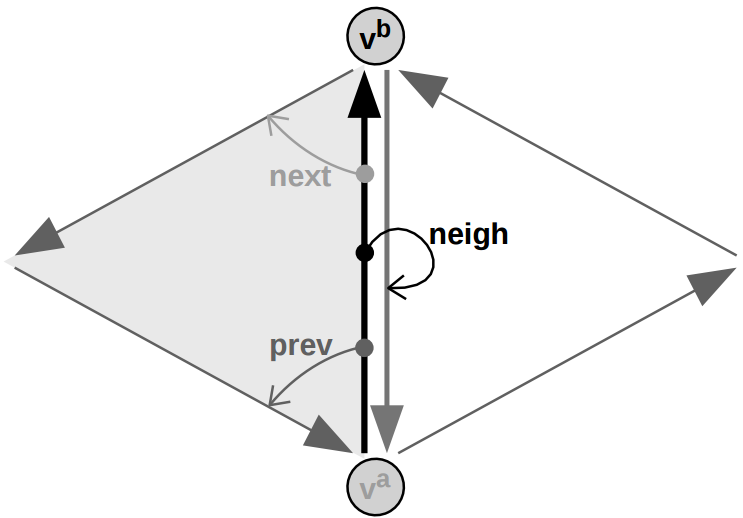
\includegraphics[width=0.45\linewidth]{images/directed-edge0.png}\hfill
   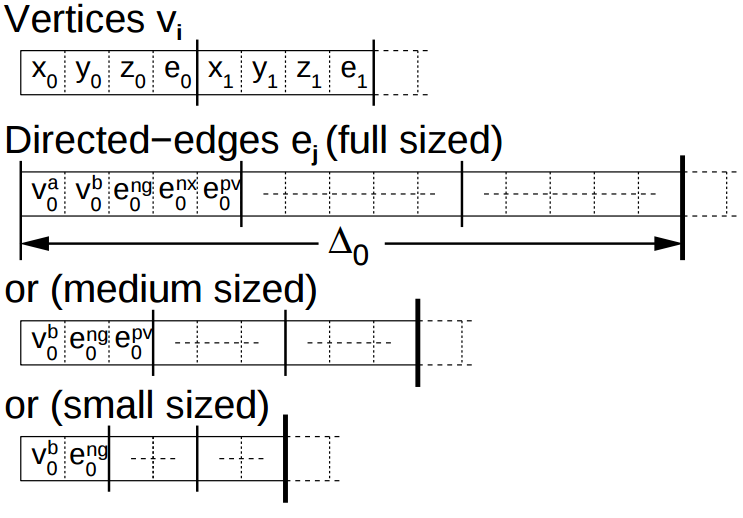
\includegraphics[width=0.45\linewidth]{images/directed-edge1.png}
   \caption[The directed-edge structure]{The directed-edge structure (a) A simple drawing of two triangular meshes with the interesting values for the data structure. Grey values can be exchanged with further computations (b) The three variants of the directed-edge data structure (note the different memory occupation). Images taken from~\cite{Campagna}}
   \label{fig:directedEdge}
\end{figure}

However, as we have seen above we can have non-manifold vertices and edges in many applications. So \cite{Campagna} introduced little modifications to this structure assuming that the number of non-manifold entities is typically 
negligible compared to the complexity of the whole mesh. We can use the following strategy:
\begin{itemize}
 \item For every couple of edges that represent a 2-manifold interior edge we can use zero or positive indexes.
 \item A directed edge on boundary is marked with a negative entry for $e^{ng}$
 \item Remembering that a 2-manifold vertex references one of its emanating edges, we can use the same strategy for non-manifold vertices and edges. A negative array-index indicates such a node and we can use this value to index a separated array which lists either all edges emanating from that vertex or the connected components attached to that vertex (as we can see in Figure~\ref{fig:directedEdge2})
\end{itemize}

\begin{figure}[htb] %  figure placement: here, top, bottom
   \centering
   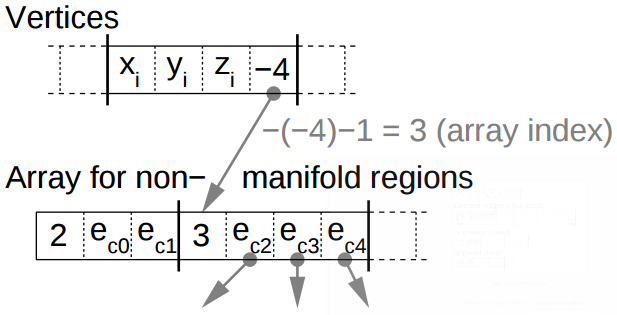
\includegraphics[width=0.45\linewidth]{images/directed-edge2.png}
   \caption[The directed-edge structure for non-manifold vertices and edges]{The directed-edge structure for non-manifold vertices and edges. Image taken from~\cite{Campagna}}
   \label{fig:directedEdge2}
\end{figure}

\subsection{Winged-edge structure}

Now we will see one of the oldest data structures proposed for mesh representation which was introduced by~\cite{Baumgart}: the \textbf{winged-edge structure}.\\
This structure explicitly describes the geometry and the topology of faces, edges and vertices when three or more surfaces share a common edge. Here is important to remember, that faces are ordered counter-clockwise with the respect of the innate orientation of the intersection edge. For this structure we need to save:
\begin{itemize}
 \item Vertices of an edge $e$
 \item Left and right faces of $e$
 \item The predecessor and the successor of $e$ when traversing its left face
 \item The predecessor and the successor of $e$ when traversing its right face
\end{itemize}

In Figure~\ref{fig:winged-edge} there is the representation schema.

\begin{figure}[htb] %  figure placement: here, top, bottom
   \centering
   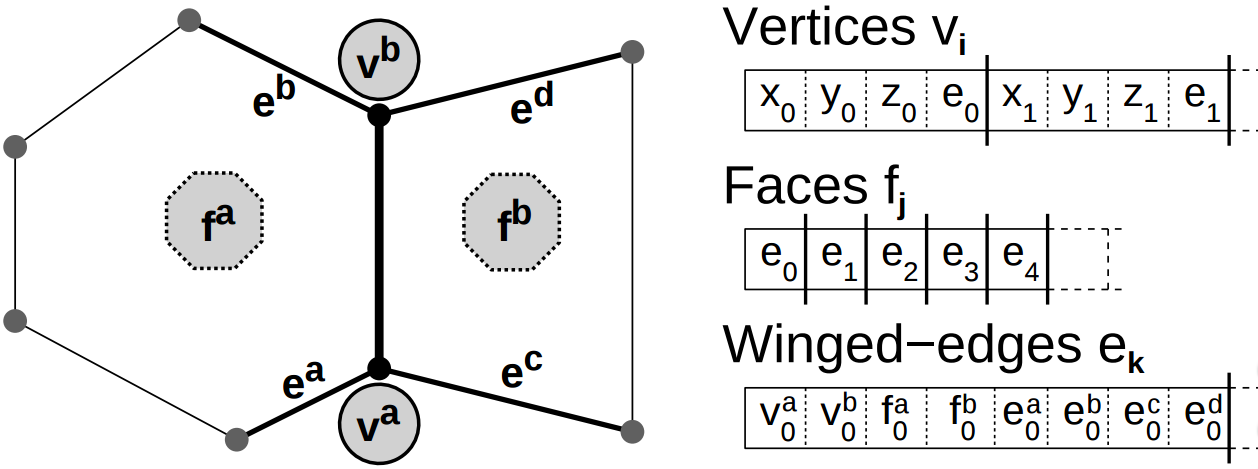
\includegraphics[width=0.60\linewidth]{images/winged-edge.png}
   \caption[The winged-edge structure]{The winged-edge structure. Image taken from~\cite{Campagna}}
   \label{fig:winged-edge}
\end{figure}

How we can see, we need three arrays to memorize all informations about our meshes. In particular, observing the Figure~\ref{fig:winged-edge} we can say that $e^a$, $e^b$ and $e^d$ are the \textit{wings} of edge $v^{a}v^{b}$ which is called \textit{winged}. This data structure is interesting because we can easily compute the relationships of adjacency between structures (some even in constant time).


\subsection{Quad-edge structure}

The \textbf{quad-edge data structure} has been introduced by \cite{Guibas} and is a representation of the topology of a two-dimensional or three-dimensional map (which is a graph drawn on a closed surface). In this structure, we represent simultaneously the map, its dual and mirror image. The main idea behind the quad-edge structure, is the recognition that an edge in a closed mesh topology sits exactly between two faces and two vertices. As a consequence, it can represent a dual of the graph simply reversing the convention on what a vertex is and what a face. However, given this definition, we have that the quad-edge can only represents manifold edges. It is easy to use this structure iteration through the topology, so it can be useful for computation of adjacency relationships.

\subsection{Half-edge structure}

The \textbf{half-edge structure} (also known as \textbf{doubly connected edge list} or \textbf{DCEL}) has been introduced by \cite{Muller} and has been designed to represent an embedding of a planar graph in the plane and polytopes in three-dimension. This data structure provides efficient manipulation of the topological information associated with the various objects (vertices, edges and faces); so it is commonly used to handle polygonal subdivisions of the plane (for example for computation of a Voronoi diagram). In the general case, a DCEL contains a record for each edge, vertex and face of the subdivision, and each record may contain additional information. As each edge usually bounds two faces, it is convenient to refer to an edge as two half edges. Each one bounds a single face and has a pointer to that face; so we can go to the other half-edge and traverse the other face. Moreover, each half-edge has a pointer to its origin vertex.\\
In addition, each vertex contains its coordinates and a pointer to an arbitrary edge that has the vertex as its origin, and each face stores a pointer to some half-edge of its outer boundary. It also has a list of half-edges, one for each hole that may be incident with the face; however, if the vertices of faces do not hold useful information we can save space by avoiding to store them.

\begin{figure}[htb] %  figure placement: here, top, bottom
   \centering
   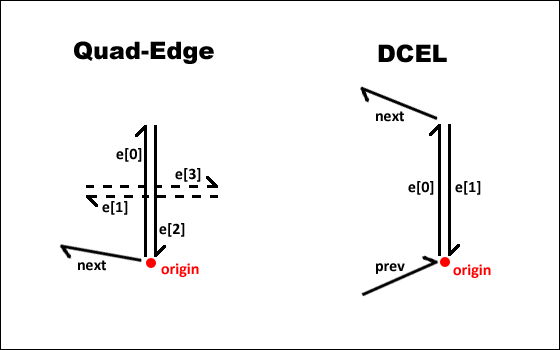
\includegraphics[width=0.60\linewidth]{images/dcel-quadedge.png}
   \caption[Comparison between the quad-edge and half-edge structures]{Comparison between the quad-edge and half-edge structures. Image taken from https://code.google.com/archive/p/cgprojects09/}
   \label{fig:dcel-quadedge}
\end{figure}

\subsection{Memory requirements for mesh structures}\label{sec14:MemoryReq}

As we have seen in previous chapters, our aim is the manipulation of great volumes of data, so as size is an important variable, we need to study the memory requirements for the structures we have studied so far.\\

The simplest data structure is based on a list of vertices and a list of faces. Assuming that each integer is stored with four bytes, this representation uses $12V$ bytes for $V$ vertices and $12T$ bytes for the $T$ triangles. From the Euler's polyhedron formula we have that:
\begin{equation}
 V - E + F = 2 - 2g
\end{equation}

Where $V$ is the number of vertices, $E$ is the number of edges, $F$ is the number of faces and $g$ is the \textit{genus} of the surface (the maximum number of cuttings along non-intersecting closed simple curves, without rendering the resultant manifold disconnected). As each triangle has three edges and each edge is shared by approximately two triangles the number of edges is $\frac{3}{2}T$. So we can write:
\begin{equation}
 V - \frac{3}{2}T + T = 2 - 2g
\end{equation}

Assuming that the genus is low with respect to the number of triangles, we can write:

\begin{equation}
 V = 2 - 2g + \frac{1}{2}T \approx \frac{1}{2}T
\end{equation}

So the number of vertices is twice the number of triangles. So the total memory (in bytes) needed by the initial data structure is:

\begin{equation}
 12V + 12T = 6T + 12T = 18T
\end{equation}

For the directed-edge data structure, each vertex uses 12 bytes for coordinates and four for an edge reference (faces are not represented). In the full sized version, each directed edge contains references to two vertices and three edges, using 20 bytes while in the medium and small sized versions we have respectively 12 and 8 bytes. So the three memory costs are:

\begin{equation}
 16V + 20\cdot 3 T \approx 8 T + 60 T = 68 T \: bytes
\end{equation}

\begin{equation}
 16V + 12\cdot 3 T \approx 8 T + 36 T = 44 T \: bytes
\end{equation}

\begin{equation}
 16V + 8\cdot 3 T \approx 8 T + 24 T = 32 T \: bytes
\end{equation}

For the winged-edge structure each vertex uses 16 bytes, each face uses four bytes and each edge has four edge references, two face references and two vertex references. So we can write:

\begin{equation}
 16 V + 32 E + 4T \approx 8T + 32 \frac{3}{2}T + 4T = 60T \: bytes
\end{equation}

We can make the same considerations for the quad-edge structure and the half-edge structure obtaining \textit{30 bytes} and \textit{38 bytes} for each triangle.\\

Finally, we can observe the Table~\ref{tbl:meshStructures} from \cite{Campagna}, where the main aspects about memory used and time spent for the main relationships computations are summarized

\begin{table}[htbp]
\centering
\caption[Comparison of several data structures]{Comparison of several data structures. "M" indicates entities that are explicitly stored, "C" means that the information may be calculated in $O(1)$, and "-" marks entities that require computations of complexity $\gg O(1)$}
\label{tbl:meshStructures}
\begin{tabular}{p{4.3cm} || p{1.3cm} | p{1.5cm} | p{1cm} | p{1.2cm} | p{0.8cm} | p{0.8cm}}
\toprule
\textbf{Data structure}	& \textbf{bytes/$\bigtriangleup$}	&\textbf{Supports non-manifold}	&\textbf{neigh-bor-hood}	&\textbf{point reference}	&\textbf{prev. edge}	&\textbf{next edge}\\ \midrule \midrule
Individual triangles              & 36	& yes	&-	&-	&(M)	&(M)\\ \midrule
shared vertex              & 18	& yes	&-	&M	&(M)	&(M)\\ \midrule \midrule
shared vertex with neig.              & 32	& no	&M	&M	&(M)	&(M)\\ \midrule
winged-edge              & 60	& no	&M	&M	&M	&M\\ \midrule \midrule
full directed-edge              & 68	& yes	&M	&M	&M	&M\\ \midrule
medium directed-edge              & 44	& yes	&M	&M,C	&M	&C\\ \midrule
small directed-edge              & 32	& yes	&M	&M,C	&C	&C\\
\bottomrule
\end{tabular}
\end{table}

\section{Volume rendering techniques}\label{sec14:volumeRendering}

\textbf{Volume rendering} techniques are used for visualization of a two-dimensional projection of a three-dimensional \textit{discretely sampled data set} (which is a \textit{three-dimensional scalar field}). A typical example of these scalar fields is represented by 2D slice of medical images (seen in Chapter~\ref{Chapter13}) which are also called \textit{range images}. \cite{Curless} points out a set of desirable properties for a volume rendering algorithm which we will report here:

\begin{itemize}
\item \textbf{Representation of range uncertainty}. The data in range images typically have asymmetric error distributions with primary directions along sensor lines of sight.
\item \textbf{Utilization of all range data}, including redundant observations of each object surface.
\item \textbf{Incremental and order independent updating}. Incremental updates allow us to obtain a reconstruction after each scan or small set of scans and to choose the next best orientation for scanning. Order independence is desirable to ensure that results are not biased by earlier scans. Together, they allow straightforward parallelization.
\item \textbf{Time and space efficiency}. Complex objects may require many range images in order to build a detailed model. So they must be represented efficiently and processed quickly.
\item \textbf{Robustness}. Outliers and systematic range distortions can create challenging situations for reconstruction algorithms. A robust algorithm needs to handle these situations without failures such as holes in surfaces and self-intersecting surfaces.
\item \textbf{No restrictions on topological type}. The algorithm should not assume that the object is of a particular genus. Simplifying assumptions such as "the object is homeomorphic to a sphere" yield useful results in only a restricted class of problems.
\item \textbf{Ability to fill holes in the reconstruction}. Given a set of range images that do not completely cover the object, the surface reconstruction will necessarily be incomplete. For some objects, no amount of scanning would completely cover the object, because some surfaces may be inaccessible to the sensor. In these
cases, we desire an algorithm that can automatically fill these holes with plausible surfaces, yielding a model that is both "watertight" and esthetically pleasing.
\end{itemize}

All algorithms for volume rendering, uses two main strategies:
\begin{itemize}
 \item Reconstruction from unorganized points
 \item Reconstruction that exploits the underlying structure of acquired data
\end{itemize}

In this section we will examine some of the most widespread techniques used for volume rendering to understand its key-features.

\subsection{Volume ray casting}

With this technique, we generate a ray for every image pixel. Using a simple \textit{camera model}, the ray starts at the center of projection of the camera and passes through the pixel on the imaginary image plane floating in between the camera and the volume to be rendered. We can save time by clipping the ray by the boundaries of the volume. The data is interpolated at each sample point, and the process repeated until the ray exits the volume. The RGBA value obtained is converted to an RGB color and saved in the corresponding image pixel. The process is repeated for every pixel on the screen to form the complete image.\\

So entering in details, we can divide the volume ray casting technique into the following four steps:
\begin{enumerate}
\item \textbf{Ray casting}. For each pixel of the final image, we cast a ray through the volume
\item \textbf{Sampling}. Along the part of the ray of sight that lies within the volume, equidistant sampling points or samples are selected
\item \textbf{Shading}. For each sampling point, a gradient of illumination values is computed. The samples are then shaded according to their surface orientation and the location of the light source.
\item \textbf{Compositing}. After all sampling points have been shaded, they are composited along the ray of sight, obtaining the final color value.
\end{enumerate}

\begin{figure}[htb] %  figure placement: here, top, bottom
   \centering
   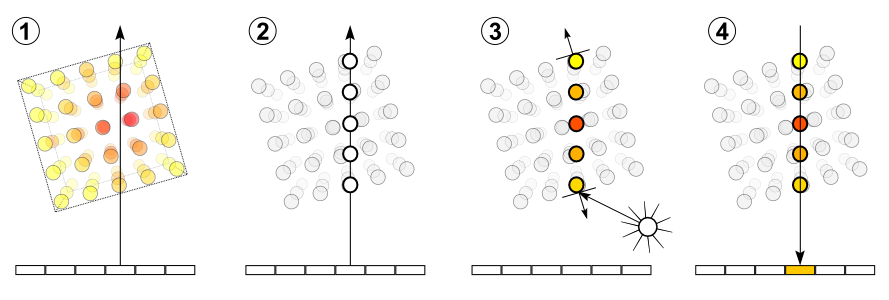
\includegraphics[width=\linewidth]{images/Volume_ray_casting.png}
   \caption[Volume ray casting]{Volume ray casting phases. (1) Ray casting (2) Sampling (3) Shading (4) Compositing. Image taken from Wikipedia}
   \label{fig:volumeRayCasting}
\end{figure}

\subsection{Maximum intensity projection}

A \textbf{maximum intensity projection} is a volume rendering method that projects, in the visualization plane, voxels with maximum intensity that fall in the way of parallel rays traced from the viewpoint to the plane of projection. This technique is computationally fast but the two-dimensional results do not provide a good sense of depth of the original data. To improve the sense of 3D, animations are usually rendered using several frames, creating the illusion of rotation

\begin{figure}[htb] %  figure placement: here, top, bottom
   \centering
   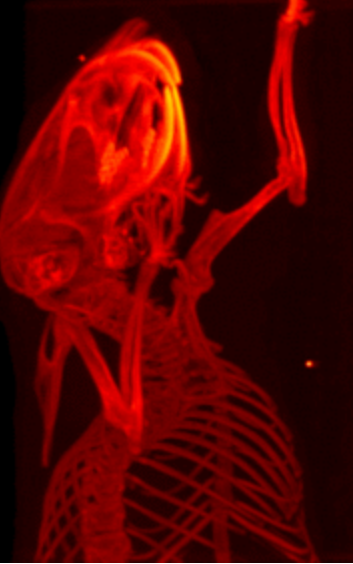
\includegraphics[width=0.25\linewidth]{images/MIP0.png}\hfill
   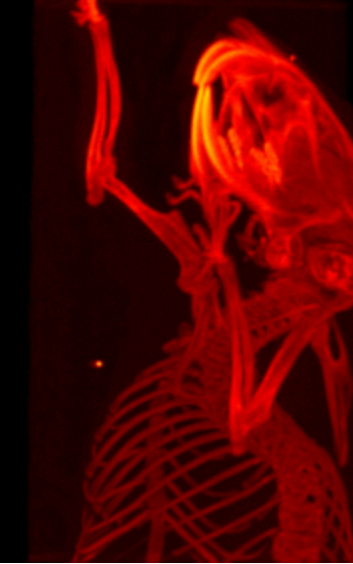
\includegraphics[width=0.25\linewidth]{images/MIP1.png}\hfill
   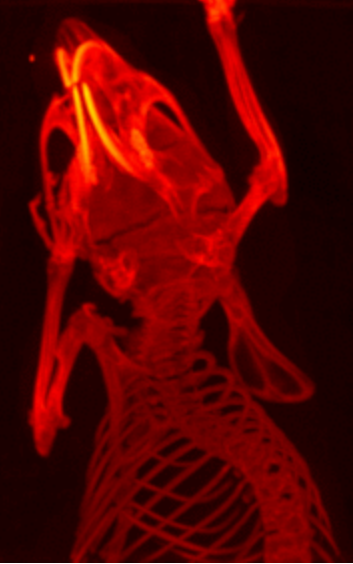
\includegraphics[width=0.25\linewidth]{images/MIP2.png}
   \caption[Maximum intensity projection]{Maximum intensity projection. From (a) to (c) different views of a MIP of a mouse  Images taken from Wikipedia}
   \label{fig:MIP}
\end{figure}

\section{Marching Cubes and iso-surfaces for data visualization}\label{sec14:isosurfaces}

In the previous section, we have seen how to generate three-dimensional representations from slices of images. These procedures are simple, inherently parallel and produce high quality renderings. However, they are quite slow (we usually have a lot of rays also in regions where they are not needed). So, when working on huge data sets, we have to use other techniques for generation of three-dimensional models. The most famous, and also the one compared with our method in the next parts, is \textbf{iso-surface rendering}. It is based on transformation of volumetric data sets into a \textit{surface model}. Now, we will see some definitions so we can better understand this method.\\

First of all we can define an \textbf{iso-surface} as a surface that represents points of a constant value within a volume of space. In mathematical words \textit{it is a level set of a continuous function whose domain is three-dimensional space}. In Figure~\ref{fig:isosurface} there is an example showing an iso-value on a sample image

\begin{figure}[htb] %  figure placement: here, top, bottom
   \centering
   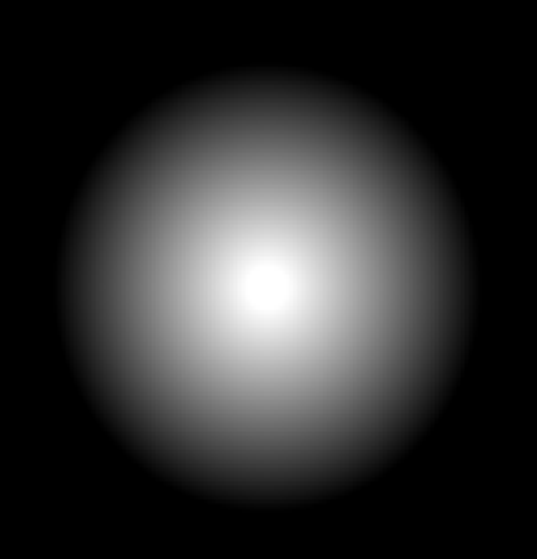
\includegraphics[width=0.35\linewidth]{images/isosurface0.png}
   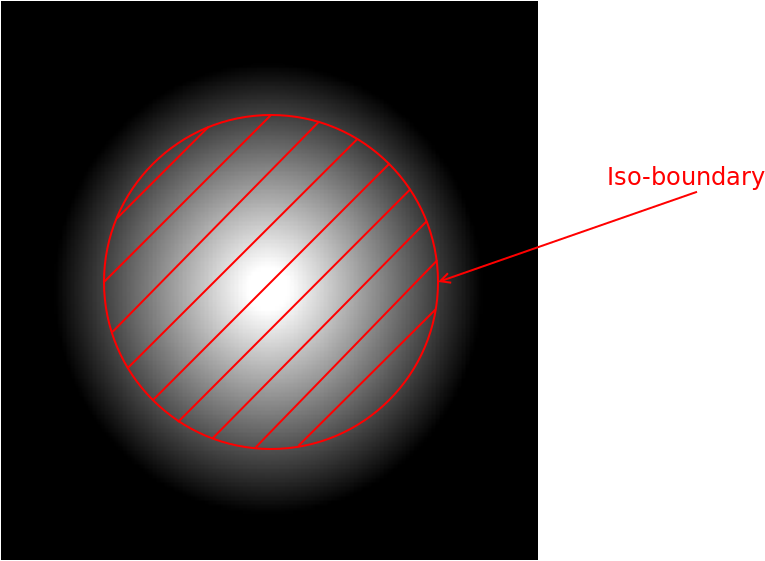
\includegraphics[width=0.45\linewidth]{images/isosurface1.png}
   \caption[Iso-boundary on a sample image]{Iso-boundary on a sample image. The chosen iso-value determines the iso-boundary (in red) and obviously the iso-surface. The rendered part of the sphere will be inside the boundary}
   \label{fig:isosurface}
\end{figure}

For the extraction of a polygonal mesh from an iso-surface, the most famous algorithm is \textbf{Marching Cubes}, which is fast and simple to implement and has been introduced by \cite{Lorensen}. A description of the algorithm is given in Listing~\ref{lst:MarchingCube}
\newpage

\begin{pseudo}[caption={Marching Cube algorithm}, label={lst:MarchingCube}]
begin
 foreach point $p$ of the scalar field:
   Take eight neighbor locations of $p$ (thus forming an imaginary cube)
 foreach cube $c$:
   if all 8 points of $c$ are above or below the iso-surface:
     ignore points
   else:
     assume surface is linear inside $c$ and emit triangles representing it 
 return mesh composed by all emitted triangles
end       
\end{pseudo}

The heart of the algorithm is in the computation of triangles into the cubes. All possible polygon configurations inside the cubes are $2^{8} = 256$, since the single vertex can either be positive or negative (above or under the surface). However, many of these are equivalent so in \cite{Lorensen} are \textit{fifteen unique cases}, which are listed in Figure~\ref{fig:MarchingCubesCases}

\begin{figure}[htb] %  figure placement: here, top, bottom
   \centering
   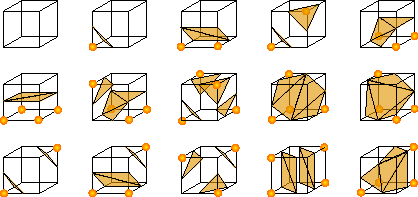
\includegraphics[width=0.60\linewidth]{images/MarchingCubes.pdf}
   \caption[All possible configurations in Marching Cubes]{All possible configurations in Marching Cubes as published by \cite{Lorensen}. The simplest pattern (the upper left one) occurs if all vertex values are above (or below) the selected value and produces no triangles. The next one occurs if the surface separates one vertex from the other seven and so on. Image taken from Wikipedia}
   \label{fig:MarchingCubesCases}
\end{figure}

So, we can generate triangles simply observing which one of the cases we have for the current cube according to the intersections of vertices with the cubes edges. However we can have problems for cases with "rippling" signs where we can have at least two correct choices for where the correct contour should pass. This problem was solved using an extended table without ambiguities that uses 33 configurations.\\

As we can see, a correct choice for the grid size has a great influence on the final result as in Figure~\ref{fig:MarchingGrid}. In fact, choosing a finer grid we have more cubes and the interpolation of surface produces a better result.

\begin{figure}[htb] %  figure placement: here, top, bottom
   \centering
   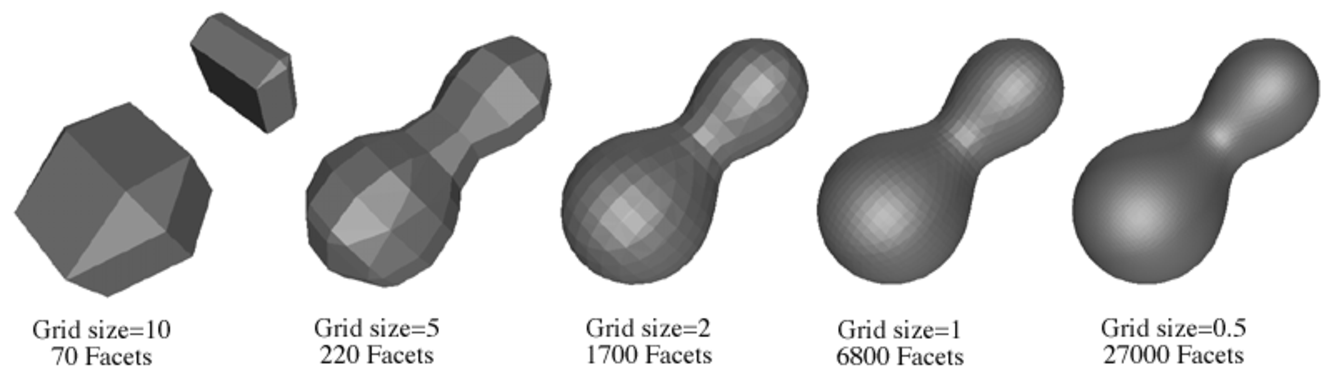
\includegraphics[width=0.90\linewidth]{images/polygoniseMarching.pdf}
   \caption[Marching Cubes grid sizes]{Marching Cubes grid sizes. How we can see in this example the final result of the Marching Cubes vary according with the grid size. Obviously choosing a finer grid we obtain a better result thus resulting in a slower computation. Image taken from \cite{Bourke}}
   \label{fig:MarchingGrid}
\end{figure}

Marching Cubes is useful for its simplicity, however despite this feature, this algorithm produces low quality meshes as we can observe in Figure~\ref{fig:MarchingQuality}

\begin{figure}[htb] %  figure placement: here, top, bottom
   \centering
   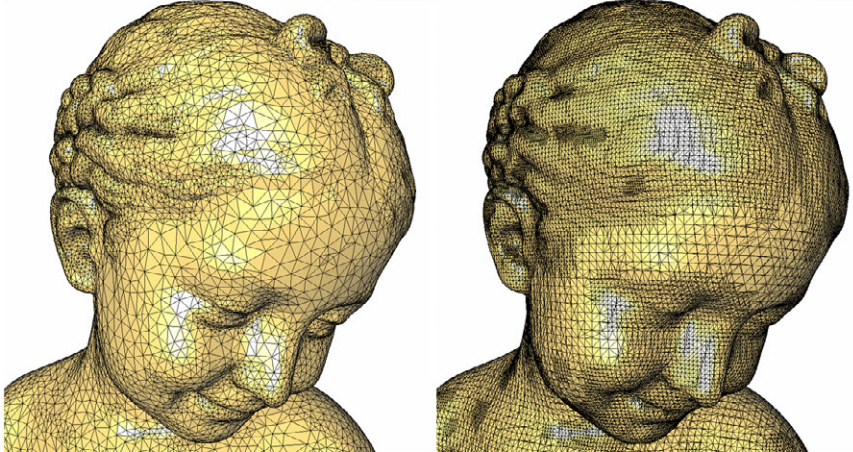
\includegraphics[width=0.50\linewidth]{images/MarchingCubeComparison.png}
   \caption[Marching Cubes quality]{Marching Cubes quality. On the left there is a model taken with an advanced reconstruction technique. On the right we have a lesser quality model taken with the Marching Cubes algorithm. Image taken from \cite{Alliez}}
   \label{fig:MarchingQuality}
\end{figure}

Another problem arises when we do not have a filled space of voxels, because any interpolated value may reduce the validity of the resulting surface. Moreover, the resulting mesh is not connected so we need to weld adjacent voxels together to get a closed mesh. Finally, we should remember that the model obtained with this method is just an approximation of the initial scalar field, in next parts we will introduce a method which will return perfect models from our data.